% Name: Topological order
% Description: Getting dressed as a directed acyclic graph, with its vertices in one topological order along a line, so that every edge points to the right.
% Tags: topological sort, DAG, ordering, dependencies

\usetikzlibrary{arrows.meta, positioning}

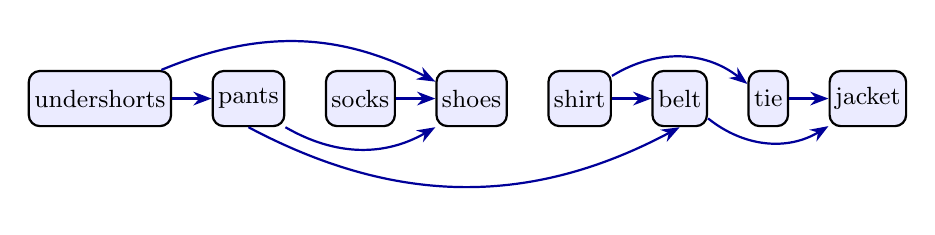
\begin{tikzpicture}[
  >={Stealth}, every edge/.style={draw, ->, thick, blue!60!black},
  task/.style={draw, thick, rounded corners, fill=blue!8, minimum height=7mm, inner sep=2pt, font=\small},
]
  \node[task] (undershorts) {undershorts};
  \foreach \t [remember=\t as \prev (initially undershorts)] in {pants, socks, shoes, shirt, belt, tie, jacket}
    \node[task, right=5mm of \prev] (\t) {\t};
  % Edges to the next vertex run straight; longer ones arc above or below without crossing.
  \path (undershorts) edge (pants)
        (socks) edge (shoes)
        (shirt) edge (belt)
        (tie) edge (jacket)
        (undershorts) edge[bend left=25] (shoes)
        (pants.south east) edge[bend right=30] (shoes.south west)
        (shirt) edge[bend left=35] (tie)
        (pants.south) edge[bend right=28] (belt.south)
        (belt) edge[bend right=35] (jacket);
\end{tikzpicture}
